
%(BEGIN_QUESTION)
% Copyright 2010, Tony R. Kuphaldt, released under the Creative Commons Attribution License (v 1.0)
% This means you may do almost anything with this work of mine, so long as you give me proper credit

Suppose we have a Siemens S7-200 PLC connected to a pair of momentary-contact pushbutton switches and light bulbs as shown in this illustration:

$$\includegraphics[width=15.5cm]{i04664x01.eps}$$

Examine the following relay ladder logic (RLL) program for this Siemens PLC, determining the statuses of the two lamps provided both switches are simultaneously pressed by a human operator:

$$\includegraphics[width=15.5cm]{i04664x02.eps}$$

Finally, draw color highlighting showing how these ``contact'' instructions will appear in an online editor program given the stated input conditions.

\underbar{file i04664}
%(END_QUESTION)





%(BEGIN_ANSWER)

If both switches are pressed, switch A will be closed ({\tt I1.2} = 1) and switch B will be open ({\tt I0.7} = 0), leading to this condition of the program:

$$\includegraphics[width=15.5cm]{i04664x03.eps}$$

Neither output will activate, resulting in both lamps de-energized.

%(END_ANSWER)





%(BEGIN_NOTES)


%INDEX% PLC, relating I/O status to virtual elements

%(END_NOTES)


